\documentclass[twocolumn]{article}
\usepackage{ctex}
\usepackage{amsmath}
\usepackage{listings}
\usepackage{graphicx}
\lstset{language=python,tabsize=4}
\usepackage{color}
\lstset{xleftmargin=-2em}
\usepackage[top=1cm,left=1.2cm,right=0.8cm]{geometry}
\title{linux脚本}
\author{W.J.Z}
\date{}
\graphicspath{{picture/}}
\begin{document}
	\maketitle
	\section{基础知识}
	1、启动一个交互式shell时,它通过执行当前用户主目录中的脚本文件$~/.bashrc$,登录shell则是$~/.bash\_profile$,Bash shell通过维护$~/.bash\_history$文件保存用户运行过的命令。
	\\

	2、打开Bash shell后,会显示如下提示符,username为当前用户名,hostname为主机名,$\$$代表一般用户,$\#$代表管理员root。
	\begin{lstlisting}
	username@hostname$
	PS1='W.J.Z>>' 可以更改显示
	\end{lstlisting}
	
	
	3、shell 脚本
	\begin{lstlisting}
	指定Bash解释器命令路径,该行
	必须在脚本的第一行
	#!/bin/bash
	赋予脚本文件执行权限
	chmod a+x sample.sh
	执行脚本
	./sample.sh 
	\end{lstlisting}
	
	4、echo使用$"",'',\quad  $三种方式终端打印时,双引号允许特殊字符的出现,如需正确输出需加转义字符。echo输出文本时自动添加换行符,添加选项$-n$可取消换行。
	\begin{lstlisting}
	echo "hello Bash shell"
	echo 'hello Bash shell'
	echo  hello Bash shell
	printf "%s" hello Bash shell
	\end{lstlisting}
	
	5、环境变量一般使用大写字母表示,其他变量使用小写字母,使用$env$可以查看当前shell所定义的全部变量。要查看其他进程变量,使用$cat \quad/proc/\$PID/environ$命令查看。
	
	\begin{lstlisting}
	查看当前shell所有的环境变量
	env  
	查看进程gedit的ID
	pgrep gedit 
	输出该进程的环境变量
	cat /proc/7405/environ | tr '\0' '\n'
	\end{lstlisting}
	
	6、重定向操作符$>> 、>$可以将输出发送到文件,前者将内容添加到文件末尾,后者先清空文件内容后写入内容。stderr标准错误输出会输入/dev/null中,该设备会丢弃接收到的任何数据。$<$读取文件的内容。
	\\
	
	7、Bash 支持普通数组和关联数组。
	\begin{lstlisting}
	定义普通数组
	array=(a b c d) 
	打印指定下标内容
	echo ${array[0]}
	打印数组中所有内容
	echo ${array[*]}
	获取数组长度
	echo ${#array[*]} 
	申明关联数组
	declare -A array
	创建关联数组
	array=([apple]='1'[banana]='2')
	查看指定索引的内容
	echo ${array[apple]}
	查看索引列表
	echo ${!array[*]}
	\end{lstlisting}
	
	8、使用alias创建别名,为使别名永久性生效,将定义添加到$~/.bashrc$中。
	\begin{lstlisting}
	alias install = 'sudo '
	\end{lstlisting}
	
	
	9、利用Bash內建的脚本调试,如果调试输出信息很长,可以重定向到文件中。
	\begin{lstlisting}
	打印执行的每一条命令以及状态
	#!/bin/bash -xv
	在执行时显示参数和命令
	set -x
	禁止调试
	set +x 
	当命令进行读取时显示输入
	set -v
	禁止打印输入
	set +v 
	\end{lstlisting}
	
	\section{文件操作命令}
	\subsection{cat命令}
	\begin{lstlisting}
	cat file1 file2 显示文件内容
	cat file1 file2 > file3 合并文件内容
	cat -s file 去掉文中空白的行
	cat -T file 将制表符显示为^I
	cat -n file 显示行号
	head -n 3 显示文件前三行
	tail -n 4 显示文件后五行
	\end{lstlisting}

	\subsection{find命令}
	\noindent find 命令参数:
	
	\begin{tabular}{|c|c|c|c|c|}
		\hline
		-type & -name & -iname & -path & -maxdepth\\
		\hline
		-mindepth &-atime & -mtime & -ctime &-amin \\
		\hline
		 -mmin & -cmin & -newer & -size &-perm \\
		 \hline
		 -exec & -and & -or & -regex & -iregex\\
		 \hline
		 !& -user & -delete & -prune & -exec\\
		 \hline
	\end{tabular}
	\\
	
	\noindent 文件类型符号:
	
	\begin{tabular}{|c|p{6.3cm}|}
		\hline
		普通文件 & f \\
		\hline
		符号链接 & l \\
		\hline
		目录 & d \\
		\hline
		字符设备 & c \\
		\hline
		块设备 & b \\
		\hline
		套接字 & s \\
		\hline
		FIFO & p\\
		\hline
	\end{tabular}
	\\
	
	\noindent 代码示例
	
	\begin{lstlisting}
	find . -name 'filename' 
	find . -type c
	find . -iname 'Filename' 忽略字母大小写
	find -L /proc -maxdepth 1 -name '1.txt'
	 2> /dev/null
	-L表示跟随符号链接 stdin(0),stdout(1)
	stderr(2)标准输入输出错误描述符标号
	find . -type f -atime -7 
	查找最近7天内被访问过的所有文件,-小于
	+大于,time以天为单位,min以分钟为单位
	find . -size 2k
	文件大小单位:b、c、w、k、M、G
	find . -perm 644 打印权限为644的文件
	find . -user r -exec chown n {} \;
	find . -name '*.git' -prune -type f
	将.git目录排除在外。
	\end{lstlisting}
	\subsection{xargs命令}
	xargs命令接受来自stdin输入,将数据解析成单个元素,然后调用指定命令并将这些元素作为该命令的参数,默认执行/bin/echo。
	\begin{lstlisting}
	cat file | xargs -n 3 
	指定每次调用的参数
	cat file | xargs -d x 
	为输入数据指定自定义分隔符
	find . -name '*.doc' -print0|
	xargs -0 grep image
	文件名中如有空格,则使用-print0
	和-0参数。
	\end{lstlisting}
	\subsection{tr命令}
	\begin{lstlisting}
	tr '\0' '\n'
	tr -d '[set1]'删除特定字符集合
	tr -c '[set1]'保留特定字符集合
	tr -s '\n' 删除重复出现的字符
	\end{lstlisting}
	
	\subsection{校检加密命令}
	md5sum和sha1sum程序可以对数据应用对应的算法来生成校检和。
	\begin{lstlisting}
	md5sum file >> md5.txt 生成校检码
	md5sum -c md5.txt 检验校检码
	MD5deep -rl file >> dir.md5
	计算目录所有文件校检和。-r递归遍历
	-l使用相对路径。
	gpg -c filename 加密文件
	gpg gilename.gog 解密文件
	\end{lstlisting}
	\subsection{行排序}
	sort和uniq命令可以从特定文件或stdin中获取输入,并将输出写入到stdout。 
	\begin{lstlisting}
	sort file1.txt file2.txt > file3.txt
	排列一组文件
	sort -n file.txt 按数字顺序排序
	sort -r file.txt 按逆序排序
	sort -M file.txt 按月份排序
	sort -m sort1 sort2 合并排序文件
	sort file.txt | uniq 找出不重复的行
	sort file.txt |uniq -u显示唯一的行
	sort file.txt |uniq -c 统计各行的次数
	sort file.txt |uniq -d 找出重复的行
	sort file | uniq -s 2 -w 2 
	-s 2忽略前2个字符,-w 2比较后续的2个字符
	\end{lstlisting}
	
	\subsection{后台执行}
	将程序放在后台执行具有两种方式,一为$\&$,二为使用ctrl+z,bg \%等命令操作。
	\begin{lstlisting}
	方法一:
	sh program.sh &
	方法二:
	查看后台执行的进程号
	jobs
	将后台进程n放到前台执行
	fg %n 
	将在前台的进程放到后台并挂起
	ctrl+z
	运行后台挂起的进程n
	bg %n
	前台进程终止运行
	ctrl+c 
	\end{lstlisting}
	
	\subsection{分割文件}
	\begin{lstlisting}
	split -b 1k d.file -d -a 4 split
	-b 指定每个分割文件的大小
	-d 分割文件后缀使用数字
	-a 指定后缀的长度
	split 指定分割文件的前缀
	
	按行进行分割
	split -l 10 data.file
	每个文件包含10行
	
	${VAR%.*}
	从$VAR中删除位于%右侧的通配符匹配的
	字符串,%%为贪婪模式,匹配模式从右
	到左
	
	${VAR#*.}
	从$VAR中删除位于#右侧的通配符匹配的
	字符串##为贪婪模式,匹配模式从左到右
	\end{lstlisting}

	\subsection{生成文件}
	\begin{lstlisting}
	dd if=/dev/zo of=jk bs =1M count =1
	if表示输入文件 input file
	of表示输出文件 output file
	bs指定单位块大小
	count 表示需要被复制的块数
	
	创建空白文件
	touch filename
	设置未见为不可修改
	chattr +i file 
	取消文件不可修改属性
	chattr -i  file
	
	创建符号链接
	ls -s target symbol
	\end{lstlisting}
	
	\subsection{文件比较}
	\begin{lstlisting}
	comm a.txt b.txt -1 -2 -3
	第一列只在a.txt出现的行
	第二列只在b.txt出现的行
	第三列在a.txt b.txt中都出现的行
	-1 删除第一列 -2 删除第二列
	
	diff -u file1.txt diff2.txt > vpatch
	-u 一体化输出
	进行文件修补
	patch -pl file1.txt < vpatch
	
	生成文件的差异信息
	diff -Naur dir1 dir2
	-N 将缺失的文件视为空文件
	-a 将所有文件视为文本文件
	-u 生成一体化输出
	-r 递归遍历目录下的所有文件
	
	wc -l file 统计行数
	wc -c file 统计字符
	wc -w file 统计单词数
	\end{lstlisting}
	
	\subsection{文件权限所有权}
	\begin{lstlisting}
	chmod 设置文件权限
	chmod u=rwx,g=rw,o=r filename
	u:用户权限 g:用户组权限 
	o:其他用户权限
	给所有用户添加可执行权限
	chmod a+x filename
	r:读权限 4
	w:写权限2
	x:执行权限1
	
	chown更改所有权	
	chmod 777 -R .
	-R 以递归的方式修改权限
	\end{lstlisting}
	
	\subsection{路径切换}
	\begin{lstlisting}
	只涉及两个位置
	cd ./
	涉及多个位置
	压入并切换路径
	pushd /var
	再压入一个路径
	pushd /tmp
	查看压入的路径
	dirs
	切换到任意路径
	pushd +0
	删除指定的路径
	popd +1
	\end{lstlisting}
	\subsection{搜索文本}
	\begin{lstlisting}{tabsize=4}
	#在stdio搜索问本行
	echo -e "hello wor"|grep wor
	#在文件中搜索问本行
	grep "mathc" file1 file2 file3
	#使用正则表达式搜搜文本
	grep -E "[a-z]" filename
	egrep "[a-z]" filename
	#只输出匹配到的文本
	grep -o "text" filenmae
	#输出不匹配的文本
	grep -v pattern file
	#输出匹配字符串所在的行号
	grep pattern -n
	#在目录中进行递归搜索
	grep pattern dir -R -n
	#忽略模式大小写
	grep -i pattern
	#指定多个模式
	grep -e pattern1 -e pattern2
	#指定搜索文件
	grep pattern file --include filename
	#排除文件
	grep pattern file --exclude filename
	#打印匹配后的n行
	grep pattern filename -A n
	#打印匹配前的n行
	grep pattern filename -B n
	#打印匹配前后的n行
	grep pattern filename -C n
	\end{lstlisting}
	\subsection{按行切分文件}
	\begin{lstlisting}
	#指定分隔符,指定提取列
	cut -f 2,3 -d "," filename
	#提取前n个字符
	cut -c -n filename
	#提取后n个字符
	cut -c n- filename
	#提取n-m个字符
	cut -c n-m filename
	\end{lstlisting}
	\subsection{sed替换文本}
	\begin{lstlisting}
	#文本替换
	sed 's/pattern/replace_str/g' file
	#使用替换的数据替换原始文件
	sed -i 's/text/replace/g' file
	#替换第n次出现的匹配
	sed 's/pattern/replace/ng' file
	\end{lstlisting}
	\subsection{awk高级文本处理}
	\begin{lstlisting}
	awk
	'BEGIN{com} pattern{com} END{com}'
	#首先执行BEGIN语块中的语句
	#接着从文件或stdio读取一行
	#匹配成功执行com命令
	#读至输入流末尾,执行END语句块
	\end{lstlisting}
	awk命令是一解释器,包含一些特殊变量
	\begin{enumerate}
		\item NR:该变量相当于当前行号
		\item NF 相当于字段数量
		\item \$0 当前记录的文本内容
		\item \$1 第一字段的文本内容
		\item \$2 第二字段的文本内容
	\end{enumerate}
	\section{高级功能}
	\subsection{下载工具}
	\begin{lstlisting}
	#下载的文件名默认和url中的文件名一样
	wget url1 url2 url3...
	#输出到指定文件
	wget url -O filename
	#尝试下载次数-t 0 不断进行测试
	wget -t 4 url
	#进行限速
	wget --limit-rate 2-k url
	#断点续传
	wget -c url
	\end{lstlisting}
	\subsection{git仓库管理}
	\begin{lstlisting}
	#创建项目文件主目录
	mkdir project
	cd project
	#创建子目录.git并初始化
	git init
	#克隆远程文件
	git clone url
	#将工作代码变更添加到暂存区
	git add file
	#将变更提交到操库
	git commit
	#查看分支
	git branch
	#创建新的分支
	git checkout -b mybrandname
	#切换到之前创建的分支
	git checkout oldbrand
	3将变更合并到新分支
	git merge
	#删除分支
	git brand -d mybrand
	#创建补丁文件
	git format-patch prebrand
	#运用补丁
	git apply --check patch
	#将分支推送到主线
	git push origin mybrand
	#更新仓库不会修改当前工作代码
	get fetch origin
	#更新仓库并修改当前代码
	git pull origin
	#查看git仓库状态
	git status
	#查看git历史记录
	git log 
	#查看Bug
	#找出引发问题的提交
	git bisect
	#快照标签
	#查看标签
	git tag
	#删除标签
	git tag -d tagname
	\end{lstlisting}
	\subsection{文件压缩与备份}
	\begin{lstlisting}
	#创建归档文件
	#-c创建新的文档 -f表示归档文件名
	tar -cf output soruce
	#列出归档文件中包含的文件
	tar -tf archive.file
	#在命令输出中显示更多的信息
	tar -tvf archive.file
	#将新文件追击到已有的归档文件
	tar -rvf origial new_file
	#从归档文件提取文件到指定目录
	tar -xf archive -C /dir
	#拼接两个归档文件
	tar -Af file1.tar file2.tar
	#通过时间戳更新归档文件
	tar -uf archive file
	#从归档中删除文件
	tar -f archive --delete file
	#压缩tar归档文件,-a自动选择压缩算法
	tar -acvf archive file
	#归档时排除部分文件
	tar -cf arch * --exclude "*.txt"
	#创建压缩文件系统
	#使用squashfs创建只读型文件系统
	mksquashfs /etc con.squashfs
	#利用环回形式挂在squashfs文件
	mkdir /mnt/temp
	mount -o loop con.squashfs /mnt/temp
	\end{lstlisting}
	\subsection{网络工具}
	\begin{lstlisting}
	#显示当前网络接口配置
	ifconfig
	设置网络接口的ip地址
	ifconfig wlan0 Ip
	#列出某个域名使用的所有ip地址
	host www.baidu.com
	#显示路由表信息
	route -n
	#检查网络是否通畅
	ping www.baidu.com -c 3
	#跟踪ip路由
	traceroute Ip
	#ssh链接远程主机
	ssh username@remote_host
	#创建ssh秘钥
	#该命令会创建公钥和私钥
	#公钥必须添加到远程服务器
	#~/.ssh/authorized_keys文件中
	ssh-keygen -t rsa
	#查看开放端口与服务
	netstat -tnp
	\end{lstlisting}
	\subsection{系统监视}
	\begin{lstlisting}
	#文件或目录体积
	du -h file
	#显示磁盘可用情况
	df -h /home/
	#测量程序执行时间
	time ls
	#查看当前用户登录信息
	who
	#查看当前登录用户更详细信息
	w
	#查看系统的加电运行时长
	uptime
	#获取指定用户信息
	last username
	#进程监视
	top
	#检查文件系统错误
	fsck /dev
	#自动尝试修复错误
	fsck -a /dev
	#生成所有进程的报告
	ps -axf 
	#查看某个命令的位置
	which ls
	#查看某个命令的更多信息
	whereis ls
	#输出对命令的简短描述
	whatis ls
	#确定文件的类型
	file filename
	#强行杀死进程
	kill -9 PID
	#获取当前系统主机名
	hostname
	#输出linux系统相关信息
	uname -a
	#输出内核发型版本
	uname -r
	\end{lstlisting}
	\onecolumn
	\section{linux文件系统}
	
	根目录是整个系统最重要的一个目录,因为不但所有的目录都是由根目录衍生出来的, 同时根目录也与开机/还原/系统修复等动作有关。 由于系统开机时需要特定的开机软件、核心文件、开机所需程序、 函式库等等文件数据,若系统出现错误时,根目录也必须要包含有能够修复文件系统的程序才行。
	
	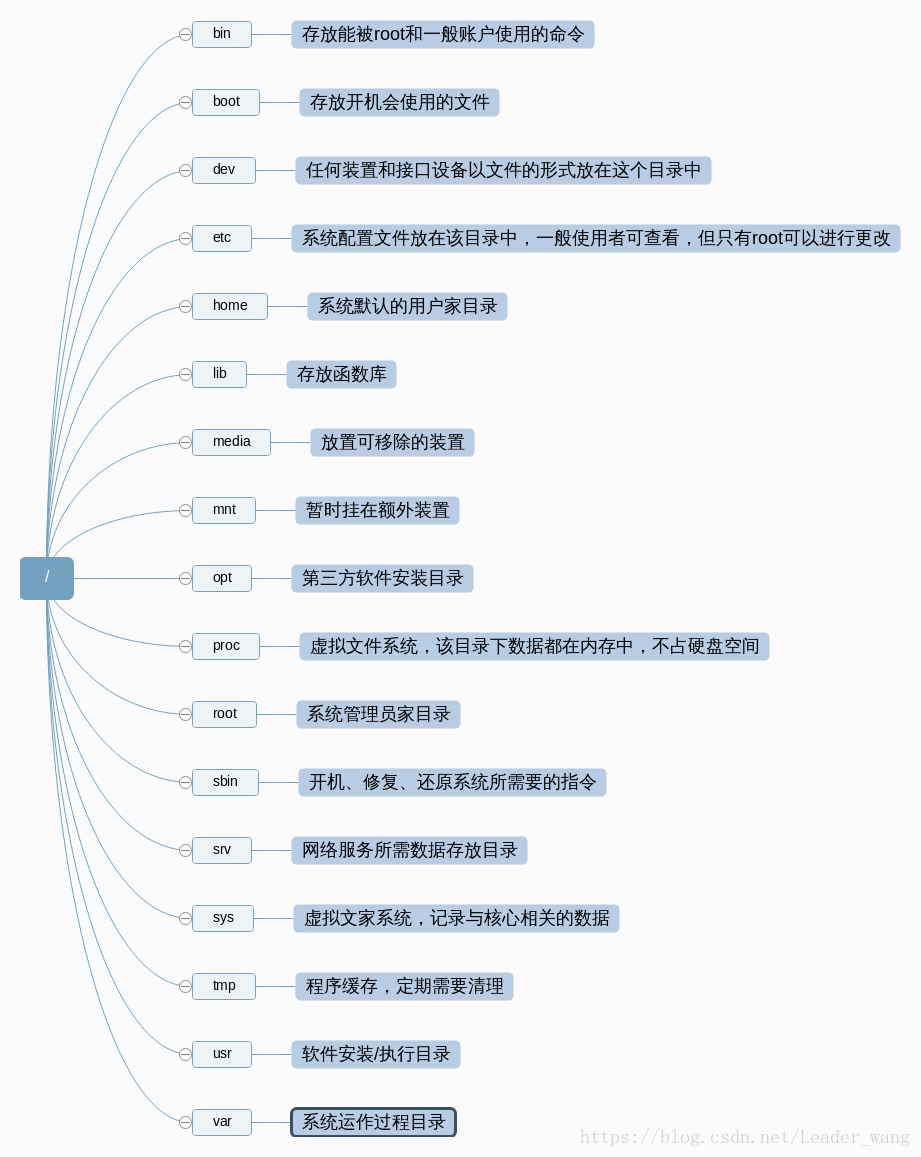
\includegraphics[width=\textwidth,height=0.75\textheight]{1}
	
	\newpage
	usr是Unix Software Resource的缩写, 也就是『Unix操作系统软件资源』所放置的目录,而不是用户的数据啦!这点要注意。 FHS建议所有软件开发者,应该将他们的数据合理的分别放置到这个目录下的次目录,而不要自行建立该软件自己独立的目录。
	
	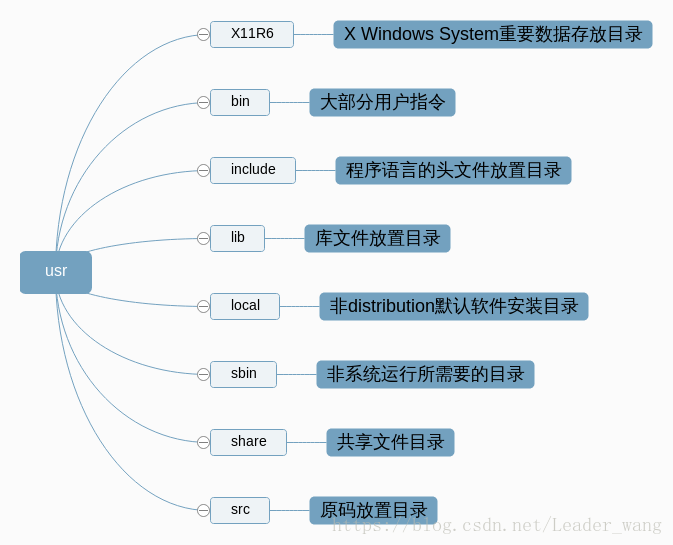
\includegraphics[width=0.8\textwidth,height=0.4\textheight]{2}
	
	/var目录主要针对常态性变动的文件,包括缓存(cache)、登录档(log file)以及某些软件运作所产生的文件, 包括程序文件(lock file, run file),或者例如MySQL数据库的文件等等。
	
	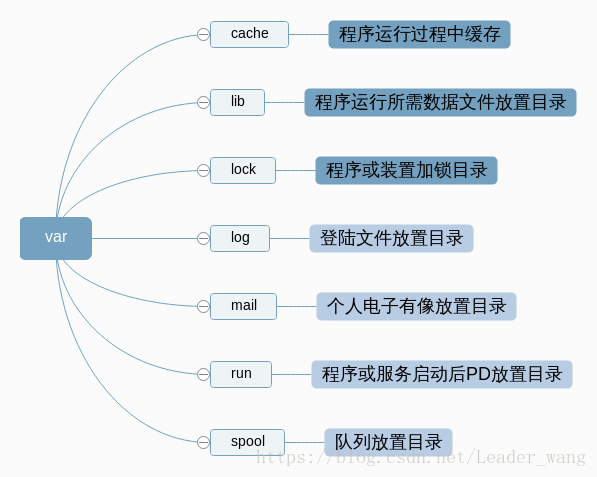
\includegraphics[width=0.8\textwidth,,height=0.4\textheight]{3}

\end{document}